\chapter{РАЗРАБОТКА ПРОГРАММНОГО ОБЕСПЕЧЕНИЯ}

\section{Требования к целевой системе}

Так как системой будут пользоваться люди, возможно, далекие от программирования, она должна иметь простой интерфейс. Система должна выводить входной текст, полученные ключевые слова и аннотацию текста. Также необходимо добавить возможность не использовать текстовые файлы, а вводить исходный текст в форму.

\section{Выбор технологий}

Для разработки алгоритмов, связанных с обработкой текста мною был выбран язык \textit{Python}. Для этого языка существует много библиотек для работы с текстами и для работы с данными. Например, для обработки текста используется библиотека \textit{nltk}. Эта библиотека предоставляет возможность загрузить словарь \quotes{стоп слов}, предоставляет необходимые функции для вычисления дистанции между словами (например функция определения косинусного расстояния \textit{cosine\_distance}). Также для реализации алгоритма \textit{Pagerank} мной была выбрана библиотека \textit{networkx}. С помощью этой библиотеки можно построить взвешенный граф по матрице расстояний и вычислить ранг каждого предложения.

Язык программирования \textit{Python} является хорошим выбором для реализации алгоритмов машинного обучения. Для него существует много высокопроизводительных библиотек для машинного обучения. Одной из таких библиотек является \textit{gensim}. Эта библиотека разработана для интерпретора \textit{CPython} и позволяет обрабатывать файлы не загружая весь файл в память.

Пользовательский интерфейс разработан на языке \textit{Javascript} с помощью библиотеки \textit{ReactJS}, которая позволяет разрабатывать одностраничные приложения. Коммуникации между модулями $mVis$ и $mControl$ происходят посредством обмена HTTP сообщениями.
В качестве библиотеки для создания HTTP сервера была выбрана библиотека \textit{Flask}.
Такой подход позволяет разместить все модули на мощном сервере, а пользователю предоставить легковесный интерфейс.

\section{Архитектура системы}

Архитектура системы включает программные модули и их отношения, представленные в моделях \hyperref[eq:scene]{(\ref{eq:scene})} и \hyperref[eq:system]{(\ref{eq:system})}. Визуально на показана на рисунке \hyperref[fig:arch]{\ref{fig:arch}}.

\begin{figure}[H]
\centering
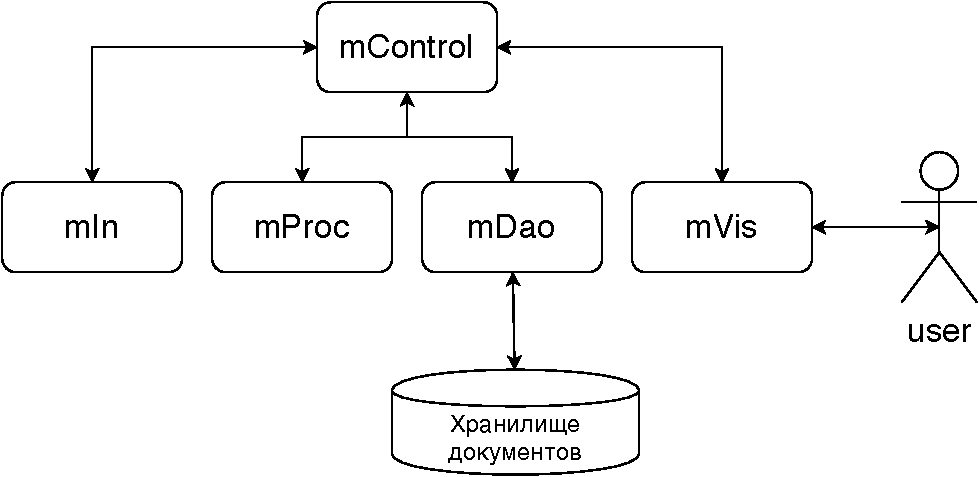
\includegraphics[width=\textwidth]{architecture.pdf}
\caption{Архитектура целевой системы}
\label{fig:arch}
\end{figure}

Формально архитектура носит жесткий характер, но обеспечивает гибкость при реализации каждого из программных модулей. Принцип построения такой архитектуры называется Low Coupling (низкое связывание). При таком подходе все модули могут разрабатываться независимо друг от друга и без больших изменений в коде программы могут добавляться новые модули.

Для того, чтобы точнее понимать, как будет работать приложение составим диаграмму последовательности для двух вариантов использования: запрос на выделение ключевых слов и составление реферата текста --- рисунок \hyperref[fig:extract]{\ref{fig:extract}}; запрос на отображение содержимого базы данных --- \hyperref[fig:fetch]{\ref{fig:fetch}}.

\begin{figure}[H]
\centering
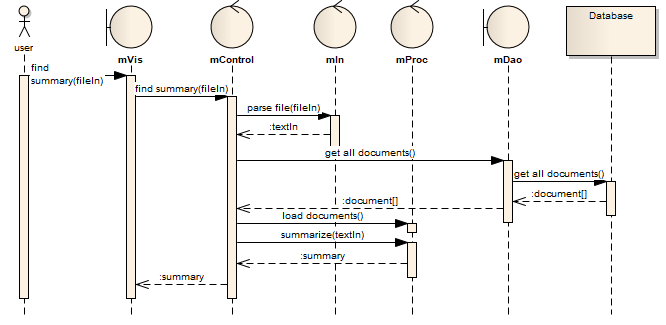
\includegraphics[width=\textwidth]{summary.png}
\caption{Диаграмма последовательности варианта использования \quotes{Выделить ключевые слова и составить аннотацию текста}}
\label{fig:extract}
\end{figure}

\begin{figure}[H]
\centering
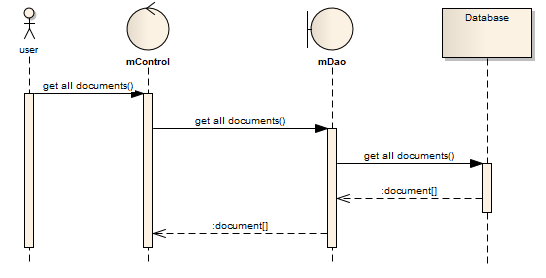
\includegraphics[width=\textwidth]{fetch.png}
\caption{Диаграмма последовательности варианта использования \quotes{Получить все документы}}
\label{fig:fetch}
\end{figure}

\section{Разработка программных модулей}

\subsection{Разработка программного модуля mProc}

Для разработки программного модуля $mProc$ использовался язык программирования $Python$. Модуль состоит из трех компонент:
\begin{itemize}
\item компонента для нахождения ключевых слов с помощью эвристического алгоритма;
\item компонента для нахождения ключевых слов с помощью алгоритма на основе модели $TF*IDF$;
\item компонента для составления аннотации текста.
\end{itemize}

При разработке использовались этого модуля для всех компонент использовались библиотека $nltk$ (Natural Language Processing Tool), которая реализует функцию нахождения косинусного расстояния, необходимую для реализации алгоритма составления аннотации текста, описанного в главе \hyperref[sec:textrank]{\ref{sec:textrank}}. Также все компоненты этого модуля используют базу данных \quotes{стоп слов}, предоставляемую этой библиотекой.
Исходный код компонент для нахождения ключевых слов с помощью эвристического алгоритма и составления реферата текста можно найти в моем репозитории на GitHub по следующей ссылке: \url{https://github.com/geobreze/summarizer/blob/master/application/api/text_rank_sum.py}.

Компонента, которая находит ключевые слова на основе модели $TF*IDF$ использует библиотеку $gensim$, которая содержит в себе инструменты для работы с естественными языками на основе алгоритмов машинного обучения. При разработке этого модуля мной была использована реализация модели $TF*IFD$, предлагаемая данной библиотекой. Для обучения модели использовался датасет (набор данных), состоящий из книг на английском языке, предоставляемых проектом Gutenberg \hyperref[itm:gutenberg]{[\ref{itm:gutenberg}]}.

\subsection{Разработка программных модулей mIn и mDao}

Программные модули $mIn$ и $mDao$ также разработаны на языке $Python$. Модуль $mIn$ использует стандартные возможности этого языка программирования для чтения входных данных и преобразования полученного входного файла в документ, представляемый списком из массивов слов. Где каждый массив слов --- одно предложение из текста. Также модуль $mIn$ обрабатывает входные данные и с помощью регулярного выражения \hyperref[eq:regexp]{(\ref{eq:regexp})} и стандартной библиотеки $re$ \hyperref[itm:regexp]{[\ref{itm:regexp}]} удаляет все символы, не являющиеся буквами английского алфавита.
\begin{equation}
\label{eq:regexp}
[\text{\textasciicircum}a-zA-Z]
\end{equation}

Модуль $mDao$ работает с нереляционной базой данных $mongoDB$, которая позволяет хранить документы в формате $JSON$. Этот формат представляет собой ассоциативный массив или набор данных в формате ключ:значение. Подключение к базе данных с помощью библиотеки $pymongo$, получение и запись данных представлена в листинге \hyperref[lst:pymongo]{\ref{lst:pymongo}}.

\begin{lstlisting}[language=Python, caption=Работа с базой данных mongoDB с помощью библиотеки pymongo, label=lst:pymongo]
from pymongo import MongoClient
client = MongoClient('mongodb://<login>:<pass>@<host>:<port>')
collection = client.database.collection
collection = insert_one({'key':'value', 'otherKey':'other value'})
db_items = collection.find()
print([item for item in db_items]) # prints {'key':'value', 'otherKey':'other value'}
\end{lstlisting}

Где <host> --- адрес базы данных, <port> --- порт для подключения к базе данных (обычно 27017), а <login> и <pass> --- логин и пароль пользователя базы данных соответственно.

\subsection{Разработка программных модулей mControl и mVis}

Программный модуль $mControl$ разработан на языке программирования $Python$ и представляет собой веб-приложение, написанное с помощью фреймворка $Flask$. Для внешних модулей модуль $mControl$ представляет интерфейс из двух конечных точек HTTP (HTTP endpoints): $POST /api/summary$ и $GET /api/documents$, которые отвечают за составление реферата текста и получение всех документов соответственно. Программный код для создания конечной точки $GET /api/documents$ представлен в листинге \hyperref[lst:endpoint]{\ref{lst:endpoint}}.  Этот модуль является модулем-делегатором, который не содержит в себе никакой логики, кроме вызова других модулей с инкапсулированной логикой.

\begin{lstlisting}[language=Python, caption=Создание конечной точки HTTP, label=lst:endpoint]
@app.route('/api/documents', methods=['GET'])
@cross_origin()
def get_all_documents():
    return common.get_not_train()
\end{lstlisting}

Модуль $mVis$ написан на языке программирования $JavaScript$ с помощью библиотеки $ReactJS$, позволяющей создавать одностраничные приложения, способные запускаться в веб-браузере. Для коммуникации с управляющей программой используется функция $fetch$, позволяющая делать асинхронные HTTP запросы. Код для обращения к модулю $mControl$ с помощью функции $fetch$ представлен в листинге \hyperref[lst:fetch]{\ref{lst:fetch}}. Обмен сообщениями между модулями $mControl$ и $mVis$ происходит в формате $JSON$.
\begin{minipage}[H]{\textwidth}
\begin{lstlisting}[caption=Обращение к модулю mControl, label=lst:fetch]
this.setState({loading: true}, () =>
    fetch(API_URL + "/api/documents")
        .then(r => r.json())
        .then(r => this.setState({loading: false, documents: r['documents']}))
);
\end{lstlisting}
\end{minipage}

\section{Выводы}

В третьей главе были получены следующие результаты:
\begin{itemize}
\item сформулированы требования к программному инструментарию;
\item разработана архитектура целевой системы;
\item разработан модуль $mProc$;
\item разработан модуль $mIn$;
\item разработан модуль $mDao$;
\item разработан модуль $mControl$;
\item разработан модуль $mVis$.
\end{itemize}

Результаты этой главы доступны в моем репозитории на GitHub по ссылке \url{https://github.com/geobreze/summarizer/tree/master/application}. 

\newpage